\hypertarget{section-runtime-view}{%
\section{6 Runtime View}\label{section-runtime-view}}

\hypertarget{__runtime_scenario_1}{%
\subsection{Display Product List}\label{__runtime_scenario_1}}
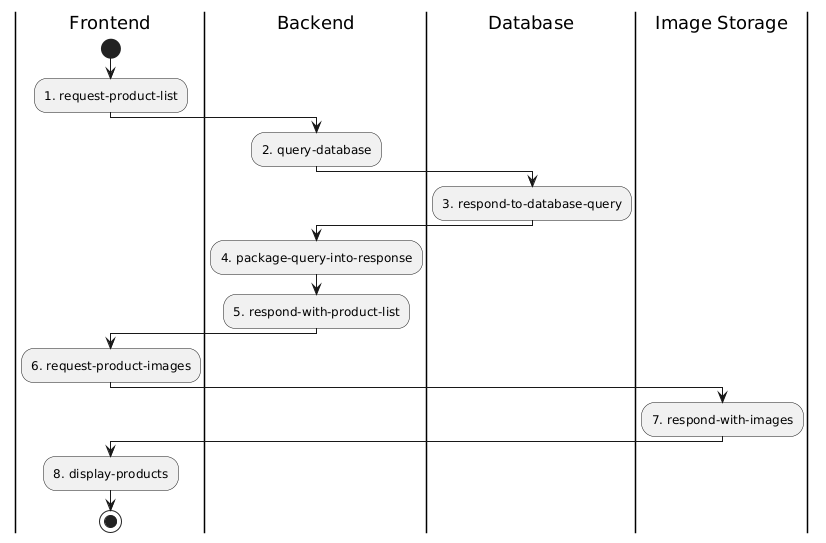
\includegraphics{images/uml_swimlane_product_list.png}

Explanation:
\begin{enumerate}
  \item Frontend request product list from backend.
  \item The backend queries the database to retrieve all the products.
  \item The database responds to the query with the products.
  \item The backend packages the result of the query into a JSON response.
  \item The backend sends the response to the frontend.
  \item 
\end{enumerate}


\hypertarget{__runtime_scenario_2}{%
\subsection{Cart Checkout Process}\label{__runtime_scenario_2}}
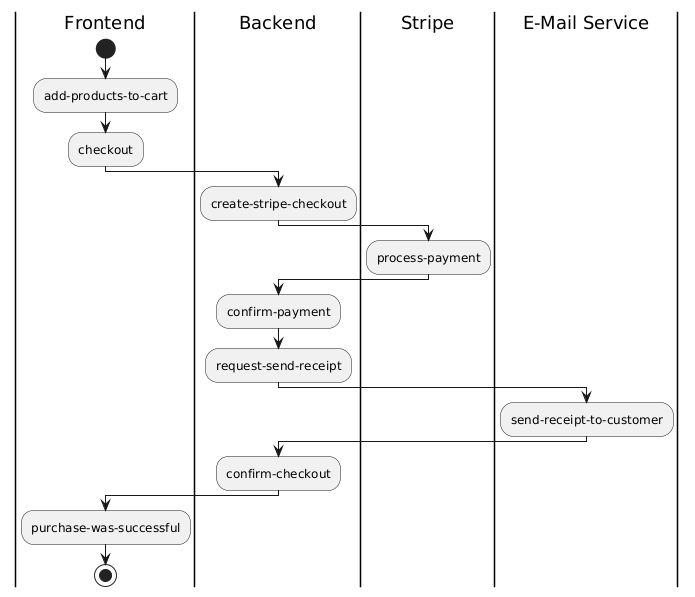
\includegraphics{images/uml_swimlane_checkout.png}

Description...

\hypertarget{__runtime_scenario_3}{%
\subsection{Creating/Updating/Deleting Products in Admin Panel}\label{__runtime_scenario_3}}
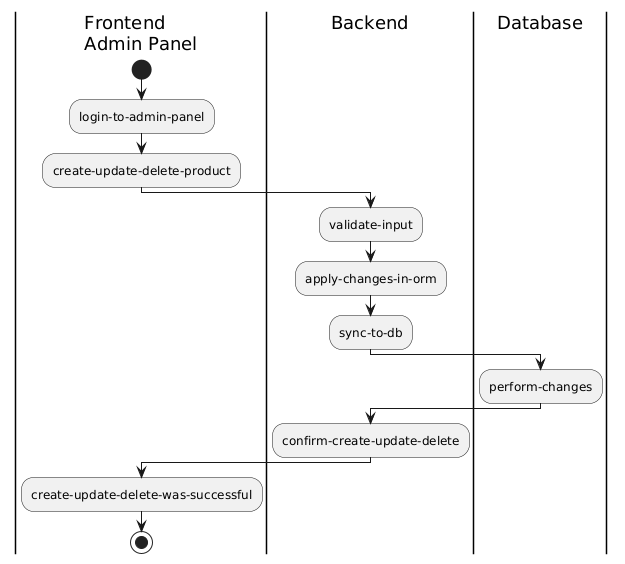
\includegraphics{images/uml_swimlane_product_create_update_delete.png}

Description...

\begin{itemize}
\item
  \emph{\textless insert runtime diagram or textual description of the
  scenario\textgreater{}}
\item
  \emph{\textless insert description of the notable aspects of the
  interactions between the building block instances depicted in this
  diagram.\textgreater{}}
\end{itemize}